\section{Momentum Experiments}

\subsection{Background}

We now consider a new network with a 785 neuron input layer, a 128 neuron
hidden layer, and a 10 neuron output layer. The hidden layer is activated by
$\tanh(\mathbf x)$ and the output with softmax. We are training for 100 epochs.

Next, we implement momentum, which inserts inertia into the movement of the weights.
Instead of the weights being updated after each batch by

\begin{align*}
	w_{t + 1} = w_t - \alpha \sum_{n = \text{start}}^{end} \nabla E^{(n)}(w)
\end{align*}

we introduce the following \textit{velocity} term $v$.

\begin{align*}
	v_n = \gamma v_{n-1} - \alpha \nabla E^{(n)}(w)
\end{align*}

which is related to the weight update rule by

\begin{align*}
	w_{t+1} = w_t + v_B
\end{align*}


where $B$ is the batch size.

Along with momentum, we implement early stopping. This technique allows us
to stop training once performance stagnates on the validation set.


\begin{algorithm}
	\caption{Neural Network Training with Early Stopping}
	\begin{algorithmic}
		\State $TODO w \gets 0$
		% \For{$t = 1$ to $M$}
		% \State Randomize the order of the indices into the training set
		% \For{$j = 1$ to $N$ in steps of B}
		% \State start = $j$
		% \State end = $j$ + B
		% \State $w_{t + 1} = w_t - \alpha \sum_{n = \text{start}}^{end} \nabla
		% 	E^{(n)}(w) $
		% \EndFor
		% \EndFor
	\end{algorithmic}
\end{algorithm}


\subsection{Performance}

Without momentum, our training and validation plots look like this


\begin{align*}
	TODO
\end{align*}

Adding momentum, with $\gamma = 0.9$, our plots now look like this

\begin{figure}[!ht]
	\centering
	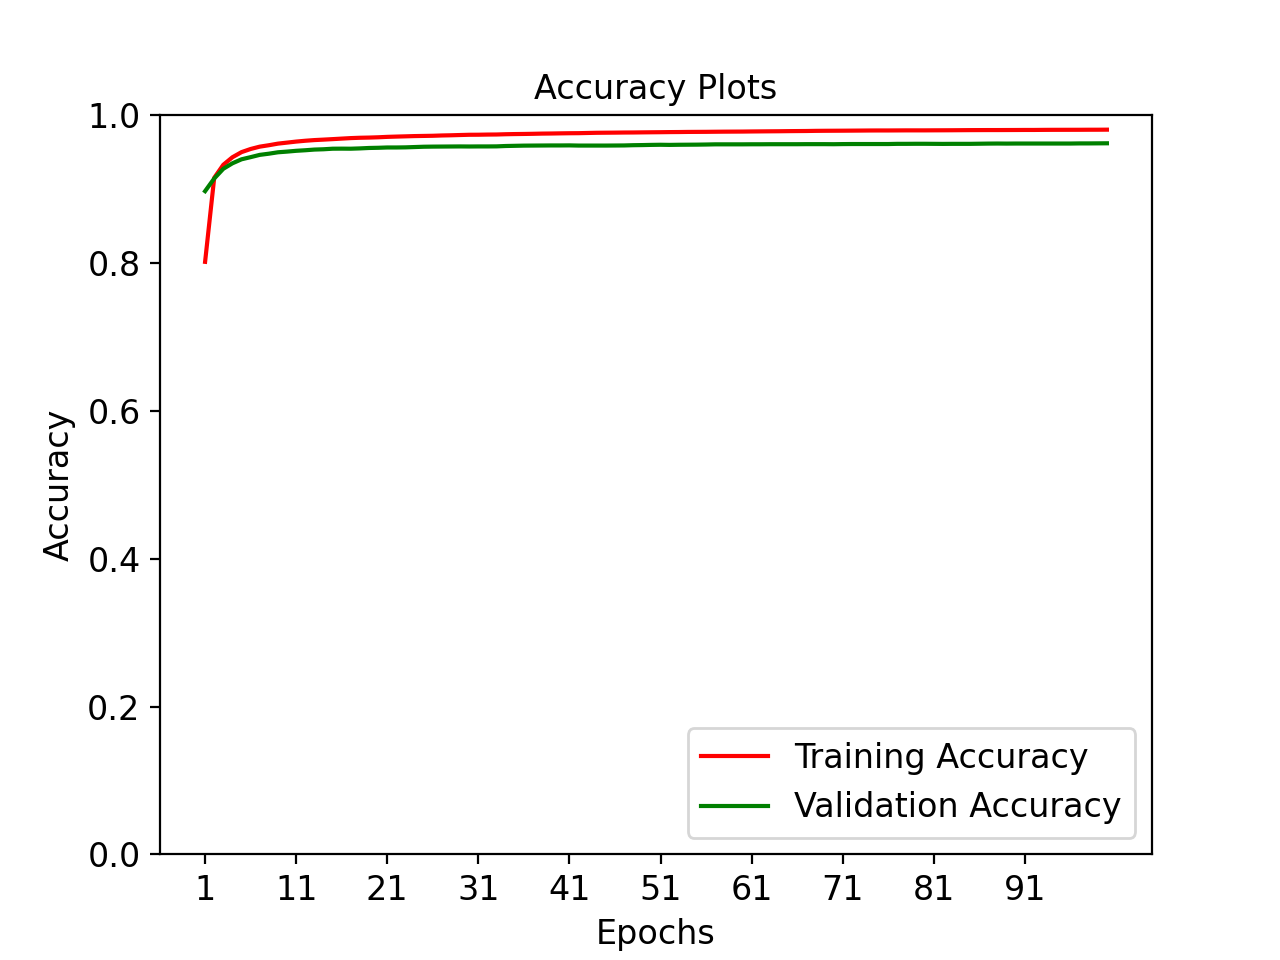
\includegraphics[width=1.0\textwidth]{./images/accuracy_momentum.png}
	\caption{Training/Validation accuracy with momentum over 100 Epochs}
\end{figure}

\begin{figure}[!ht]
	\centering
	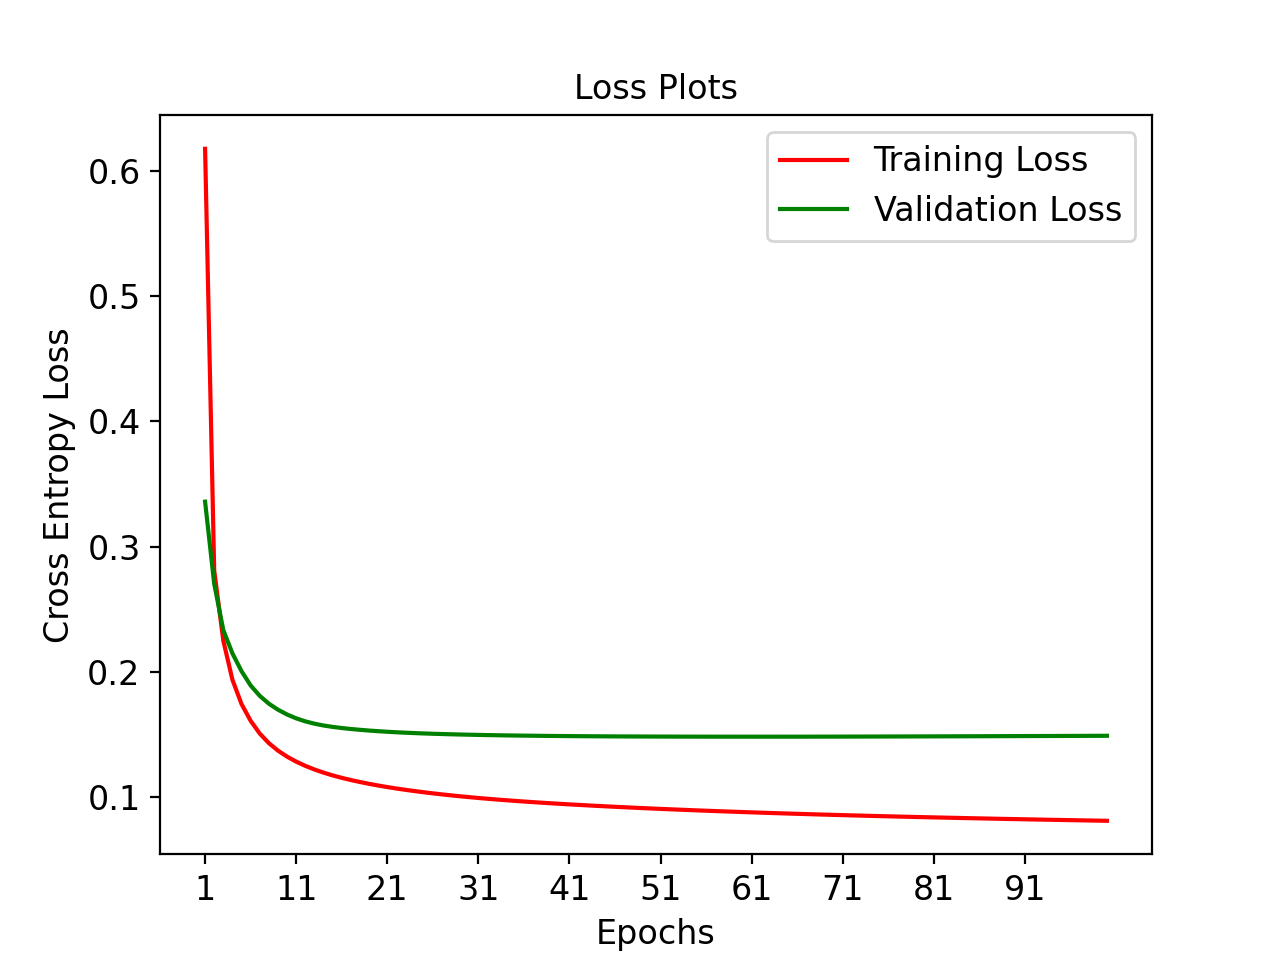
\includegraphics[width=1.0\textwidth]{./images/loss_momentum.png}
	\caption{Training/Validation loss with momentum over 100 Epochs}
\end{figure}

This model scores $96.64\%$ on the test set.


Next, we implement early stopping. We saw that 63 epochs were sufficient
for our training.

\begin{figure}[!ht]
	\centering
	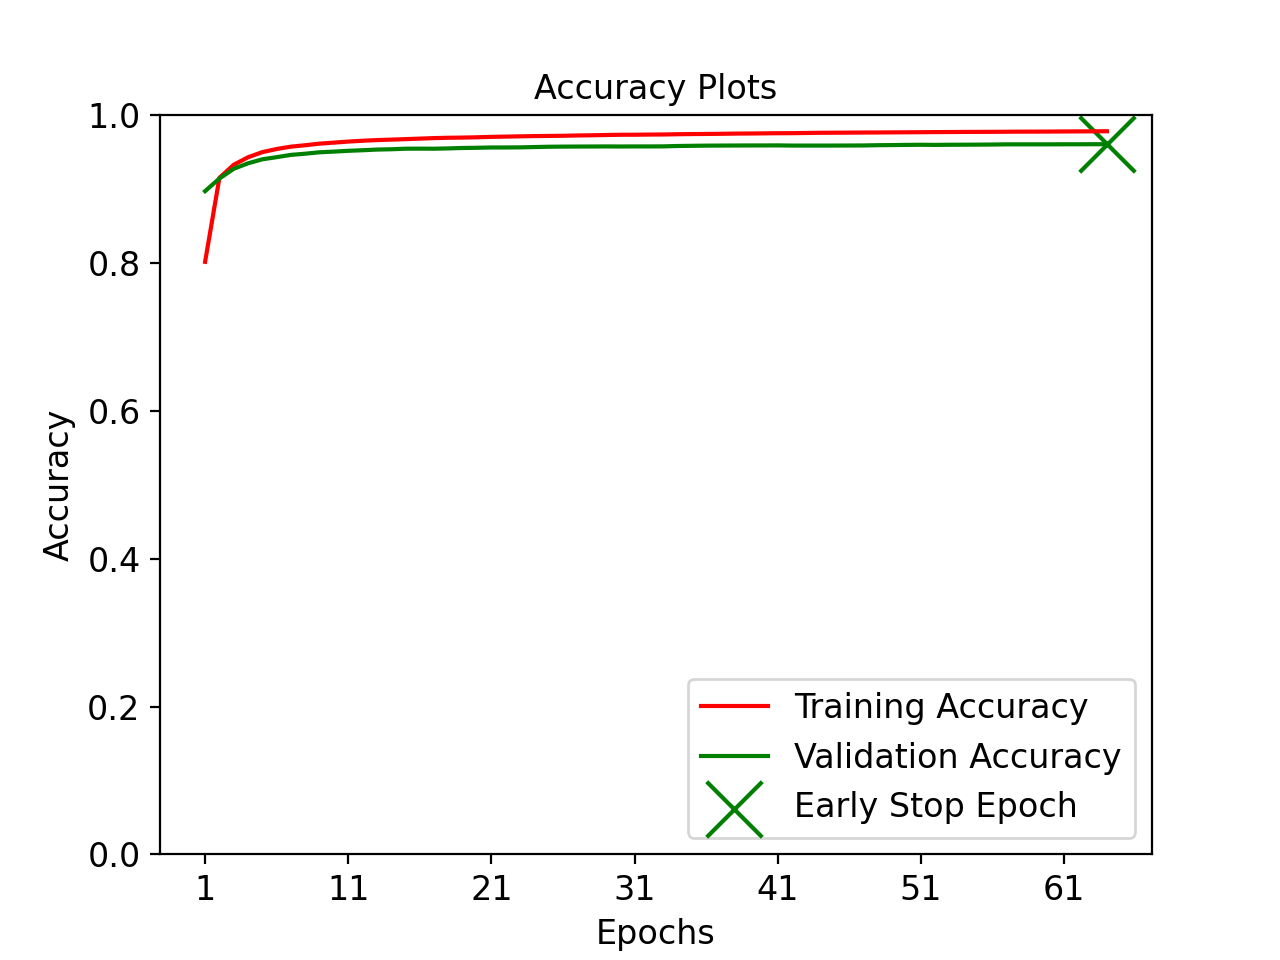
\includegraphics[width=1.0\textwidth]{./images/accuracy_momentum_early_stop.png}
	\caption{Training/Validation accuracy with momentum and early stopping}
\end{figure}

\begin{figure}[!ht]
	\centering
	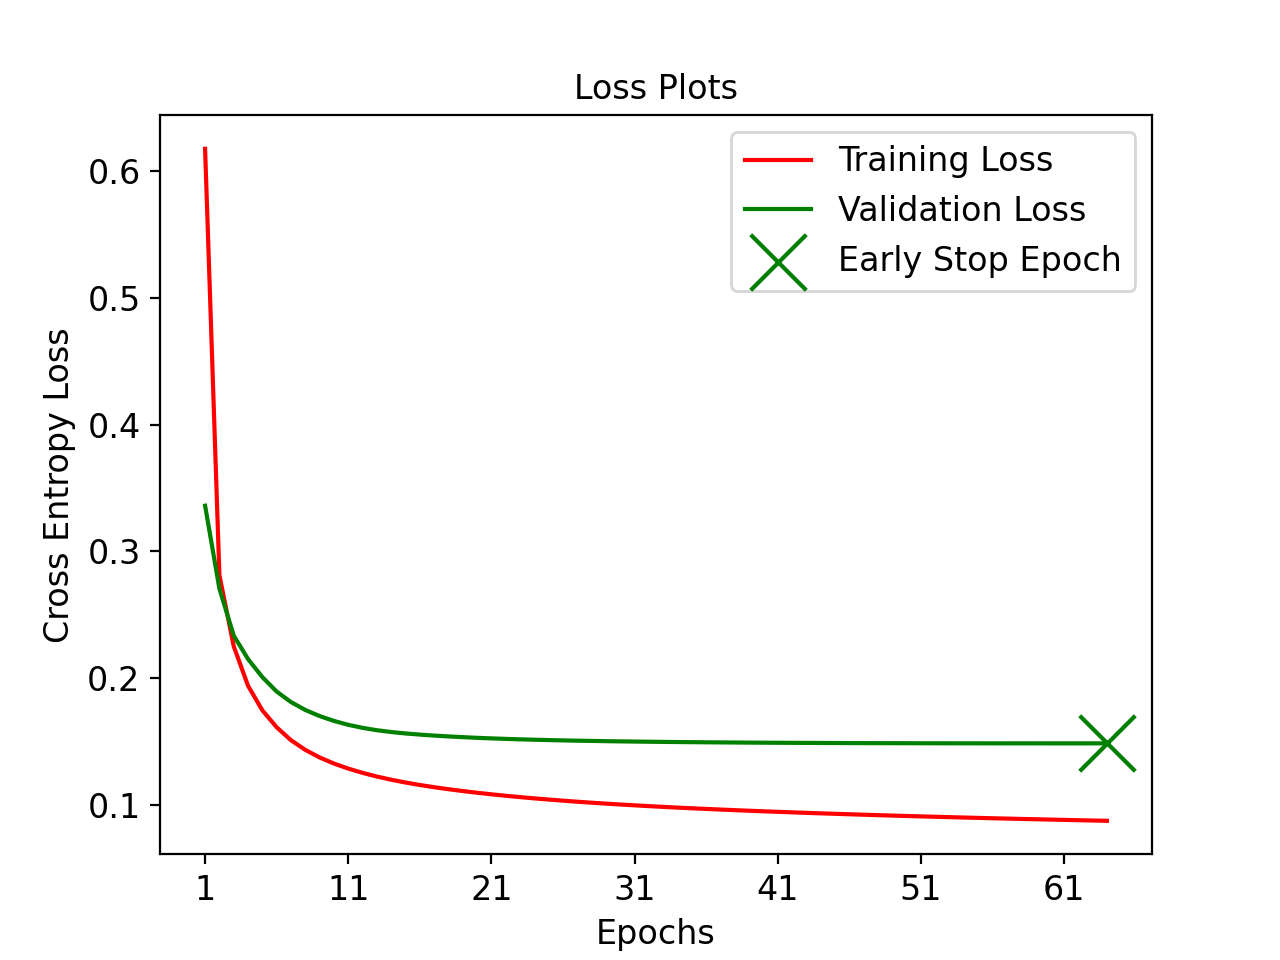
\includegraphics[width=1.0\textwidth]{./images/loss_momentum_early_stop.png}
	\caption{Training/Validation loss with momentum and early stopping}
\end{figure}

This model scores $96.56\%$ on the test set.

\subsection{Observations}

Momentum helps to smooth out noise in the gradients, especially when there are hidden layers. We also found
in testing that calculating $v$ within the batch performed significantly better than calculating $v$ after each
batch.

Early stopping is an excellent way to detect convergence, and saved us considerable training time. It also gives
an objective measure how many epochs are necessary for future training given a value of $\alpha$.
